\documentclass[12pt]{article}

\usepackage{sbc-template} 
\usepackage{graphicx,url}
\usepackage{url}
\usepackage[brazil]{babel} 
\usepackage[utf8]{inputenc} 
\usepackage[T1]{fontenc}
\usepackage[normalem]{ulem}
\usepackage[hidelinks]{hyperref}

\usepackage[square,authoryear]{natbib}
%\usepackage{amssymb} 
%\usepackage{mathalfa} 
%\usepackage{algorithm} 
%\usepackage{algpseudocode} 
%\usepackage[table]{xcolor}
%\usepackage{array}
\usepackage{titlesec}
%\usepackage{mdframed}
%\usepackage{listings}

%\usepackage{amsmath} 
%\usepackage{booktabs}

\urlstyle{same}

%\newcolumntype{L}[1]{>%{\raggedright\let\newline\\\arraybackslash\hspace{0pt}}m{#1}}
%\newcolumntype{C}[1]{>{\centering\let\newline\\\arraybackslash\hspace{0pt}}m{#1}}
%\newcolumntype{R}[1]{>{\raggedleft\let\newline\\\arraybackslash\hspace{0pt}}m{#1}}

%\newcommand\Tstrut{\rule{0pt}{2.6ex}} 
%\newcommand\Bstrut{\rule[-0.9ex]{0pt}{0pt}} 
%\newcommand{\scell}[2][c]{\begin{tabular}[#1]{@{}c@{}}#2\end{tabular}}

\usepackage[nolist,nohyperlinks]{acronym}

\title{Sistemas Especialistas}

\author{Autores: Matheus Mello e Jorge Harbes\inst{1}}


\address{Centro Federal de Educação Tecnológica Celso Suckow da Fonseca - CEFET/RJ
\email{jharbes@hotmail.com}
\email{matheusmello142012@gmail.com}
}


\begin{document} 
	
	\maketitle
	
	\begin{resumo} 
		Este artigo tem o propósito de reunir informações sobre as experiências e conhecimentos absorvidos nas aulas de sistemas especialistas, lecionada pelo professor \href{https://turing.pro.br/kadupantoja/}{Carlos Eduardo Pantoja}.
	\end{resumo}
	
	\section{Introdução}
	\label{sec:introducao}
		
    Nesta disciplina aprendemos um pouco mais sobre agentes, sistemas multiagentes, agentes cognitivos baseados em BDI e programação baseada em estímulos. O conteúdo é vasto, e as possibilidades, exponenciais. Como, por exemplo, um novo modelo de comunicação entre drones, abrindo novas possibilidades para esta tecnologia que hoje já se tornou um mercado.
    
    Utilizamos a IDE \href{https://github.com/chon-group/chonIDE}{ChonIDE}, desenvolvida pelos nossos próprios colaboradores.
	
	\section{O que é um agente ?}
	\label{sec:agente}
	
	Um agente é uma entidade autônoma e computacional que pode perceber seu ambiente, tomar decisões, agir e interagir com outros agentes para alcançar um ou mais objetivos. Normalmente é programado para que, diante de determinada análise, tome decisões baseado em conhecimentos preestabelecidos ou adquiridos. É o protagonista de todo o enredo de sistema multiagente.
	
	\section{Sistema MultiAgente}
	\label{sec:sis_multiagente}

    Um sistema multiagente é composto por vários agentes que interagem entre si para atingir objetivos individuais ou coletivos. Estes agentes podem ser tanto cooperativos quanto competitivos, dependendo da natureza do sistema e dos objetivos a serem alcançados. Cada agente em um sistema multiagente possui a capacidade de operar de forma independente, mas a interação entre os agentes é crucial para o funcionamento eficaz do sistema como um todo.
	
	\section{Agentes cognitivos em BDI}
	\label{sec:agentes_cog}

    BDI é uma abreviação de "Belief-Desire-Intention". É um modelo de arquitetura de agentes que é baseado nos conceitos de crenças (beliefs), desejos (desires) e intenções (intentions) de um agente.
    \begin{itemize}
    \item Crenças (Beliefs): São as informações que o agente possui sobre o mundo ao seu redor.
    \item Desejos (Desires): São os objetivos que o agente deseja alcançar.
    \item Intenções (Intentions): São os planos de ação que o agente decide executar para alcançar seus desejos.
    \end{itemize}

    \section{O que é AgentSpeak?}
	\label{sec:sis_multiagente}

    Agentspeak é uma linguagem de programação lógica voltada para a modelagem e implementação de sistemas multiagentes. Ela se baseia em lógica de ação, permitindo que agentes autônomos expressem suas crenças, intenções e ações de maneira formal, facilitando a comunicação e coordenação entre agentes em ambientes complexos. É amplamente utilizada em pesquisa em inteligência artificial distribuída e sistemas multiagentes. Foi criada na década de 1990 por Michael Wooldridge, Nicholas R. Jennings e David Kinny. Ela foi desenvolvida como uma linguagem de programação específica para sistemas multiagentes e desde então tem sido usada em pesquisas e aplicações na área de inteligência artificial distribuída e sistemas multiagentes.

    \section{O que é Jason?}
	\label{sec:sis_multiagente}

    Jason é uma implementação do interpretador AgentSpeak, uma linguagem orientada a agentes baseada em lógica, facilitando a criação de agentes inteligentes dentro de sistemas multiagentes (MAS). Influenciada pelo Prolog, essa ferramenta é particularmente adequada para desenvolver agentes seguindo o modelo BDI (Belief-Desire-Intention), onde os agentes possuem crenças sobre o mundo, desejos ou objetivos a serem alcançados, e intenções ou planos para alcançar esses desejos. Jason proporciona um ambiente de desenvolvimento que assiste na codificação, depuração e teste de agentes, e quando integrado aos frameworks CArtAgO e MOISE através da plataforma JaCaMo, oferece uma solução robusta para desenvolver e organizar sistemas multiagentes complexos.


    \vspace{10mm} 
    \begin{center} 
    \Large 
    \textbf{Experiência Realizada} 
    \end{center} 

    \setcounter{section}{0}
    \section{Objetivo}

    O objetivo deste projeto é desenvolver um chatbot de nível básico, que incorpora os conceitos e técnicas aprendidos na disciplina de Sistemas Especialistas. O foco será em aplicar os fundamentos de linguagens de programação e agentes inteligentes, conforme discutido nas seções anteriores do documento. Especificamente, vamos explorar a implementação de Agentes Cognitivos baseados no modelo BDI (Belief-Desire-Intention), mas em um contexto mais simplificado e direto. O uso de sistemas multiagentes ajudará a estruturar o chatbot de forma que ele possa operar eficientemente, embora em um ambiente menos complexo do que os sistemas avançados.


    \section{Metodologia}

    A metodologia para o desenvolvimento do chatbot é fundamentada nos princípios e técnicas discutidos nas seções anteriores, envolvendo uma abordagem sistemática e faseada. O processo será dividido em várias etapas principais:

    \begin{enumerate}
    \item \textbf{Planejamento e Design:} Esta fase envolve a definição clara dos objetivos do chatbot, o escopo de suas funcionalidades e a estruturação básica de como os agentes interagirão no sistema. Será desenvolvido um design conceitual do chatbot, incluindo um diagrama de como os agentes BDI irão operar e interagir dentro do sistema.

        \item \textbf{Desenvolvimento dos Agentes:} Utilizando a linguagem AgentSpeak, programaremos os agentes com capacidades específicas de percepção, raciocínio e ação. Cada agente será desenhado para realizar funções específicas dentro do chatbot, seguindo o modelo BDI, onde suas crenças, desejos e intenções guiarão seu comportamento.

        \item \textbf{Integração e Testes:} Os agentes desenvolvidos serão integrados em um ambiente de sistema multiagente, usando a plataforma Jason. Esta etapa envolve a coordenação e comunicação entre os agentes, assegurando que eles funcionem harmoniosamente. Testes iterativos serão realizados para identificar e corrigir problemas de interação e funcionalidade.

        \item \textbf{Interface de Usuário:} Desenvolvimento de uma interface de usuário amigável para permitir a interação efetiva entre o usuário e o chatbot. Esta interface será projetada para ser intuitiva, garantindo que os usuários possam se engajar facilmente com o chatbot.

        \item \textbf{Avaliação e Iteração:} Após a implementação, o chatbot será submetido a uma série de avaliações para testar sua eficácia, usabilidade e precisão nas respostas. Com base no feedback recebido, faremos as iterações necessárias para melhorar e refinar o chatbot.

    \end{enumerate}

    Essa abordagem metodológica garantirá que todos os aspectos do chatbot sejam cuidadosamente considerados e desenvolvidos, resultando em uma ferramenta interativa e eficaz que alinha os conceitos teóricos com a aplicação prática.



    \section{Implementação}

    A implementação do chatbot baseia-se nos princípios de sistemas multiagentes e na arquitetura BDI (Belief-Desire-Intention), utilizando a linguagem AgentSpeak e a plataforma Jason. O processo de implementação segue as seguintes etapas:

    \begin{enumerate}
        \item \textbf{Configuração do Ambiente de Desenvolvimento:} Inicialmente, configuramos o ambiente de desenvolvimento integrando a IDE (como ChonIDE ou similar) com a plataforma Jason. Isso nos permite desenvolver e testar os agentes em um ambiente controlado.

        \item \textbf{Criação dos Agentes BDI:} Cada agente é criado com um conjunto específico de crenças (beliefs), desejos (desires) e intenções (intentions). As crenças representam o conhecimento do agente sobre o mundo e o estado do chatbot, os desejos indicam os objetivos que o agente busca alcançar, e as intenções são os planos que o agente executa para satisfazer seus desejos.

        \item \textbf{Programação em AgentSpeak:} Utilizando AgentSpeak, programamos os comportamentos e as interações dos agentes. Isso inclui a capacidade de processar entradas do usuário, realizar raciocínio lógico, e responder apropriadamente. Os agentes são programados para serem autônomos, mas também capazes de comunicar-se e colaborar quando necessário.

        \item \textbf{Integração dos Agentes:} Os agentes são integrados em um sistema multiagente coordenado. Eles interagem entre si para compartilhar informações, tomar decisões e fornecer respostas coesas ao usuário. Esta etapa envolve a sincronização das ações dos agentes e a gestão de seus estados e interações.

        \item \textbf{Testes e Ajustes:} Após a implementação inicial, realizamos uma série de testes para avaliar o desempenho do chatbot. Isso inclui testar a precisão das respostas, a eficiência da comunicação entre agentes e a usabilidade da interface. Com base nos resultados dos testes, fazemos os ajustes necessários para melhorar a funcionalidade e a experiência do usuário.

    \end{enumerate}

    Através dessa abordagem de implementação, buscamos criar um chatbot que não apenas responda às perguntas dos usuários, mas também ofereça uma experiência interativa e enriquecedora, demonstrando os conceitos aprendidos na disciplina de Sistemas Especialistas.


    \vspace{10mm} 
    \begin{center} 
    \Large 
    \textbf{Fotos da Experiência} 
    \end{center} 

    \vspace{10mm} 
    \setcounter{section}{0}

    \section{Codificação}

    
    \begin{figure}[!ht]
        \centering
        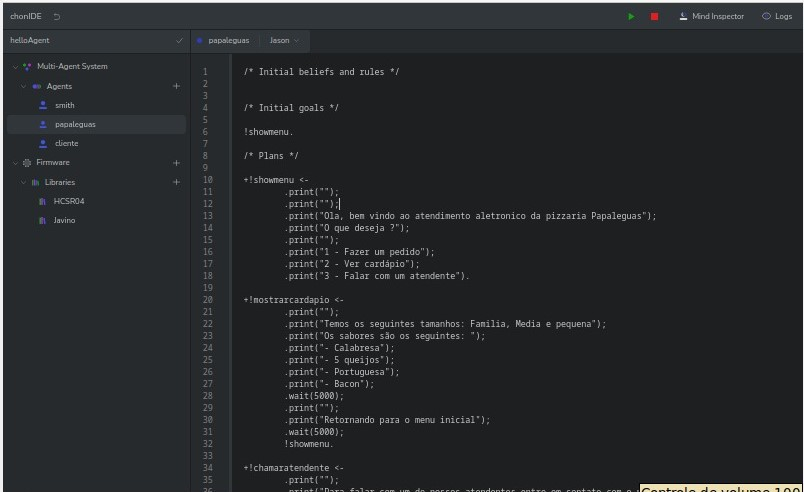
\includegraphics[width=1\textwidth]{figures/imagem05.jpeg}
        \caption{Codificação 1}
        \label{fig:imagem5}
    \end{figure}

    \begin{figure}[!ht]
        \centering
        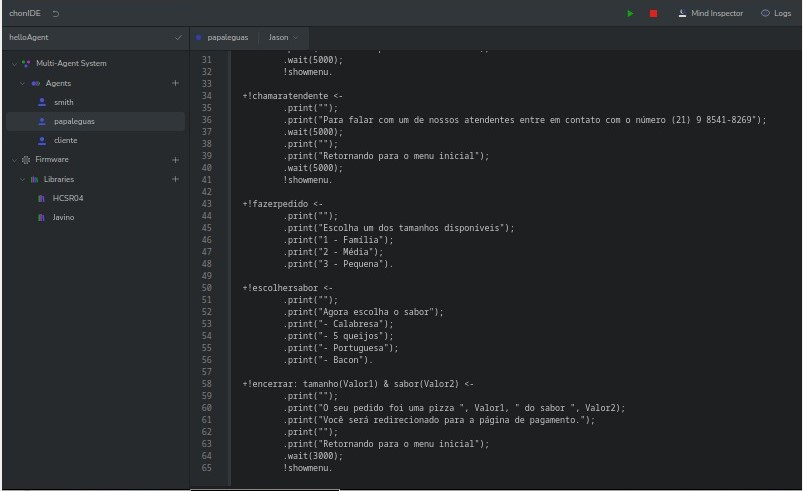
\includegraphics[width=1\textwidth]{figures/imagem06.jpeg}
        \caption{Codificação 2}
        \label{fig:imagem6}
    \end{figure}

    \newpage

    \begin{figure}[!ht]
        \centering
        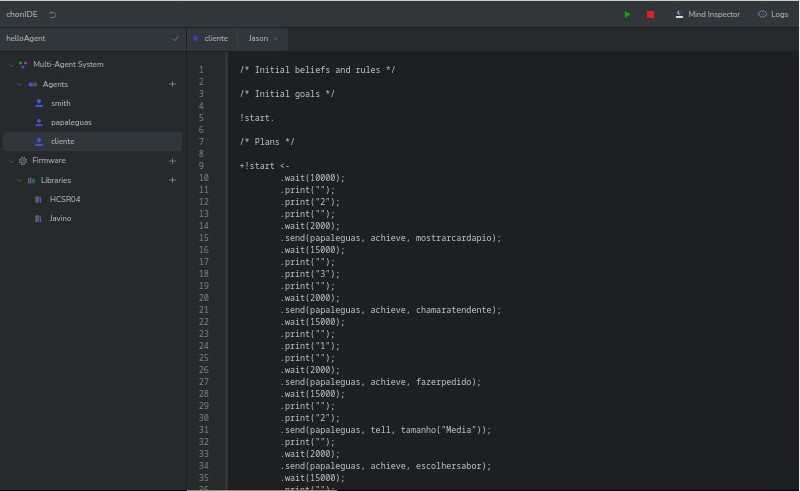
\includegraphics[width=1\textwidth]{figures/imagem07.jpeg}
        \caption{Codificação 3}
        \label{fig:imagem7}
    \end{figure}

    \begin{figure}[!ht]
        \centering
        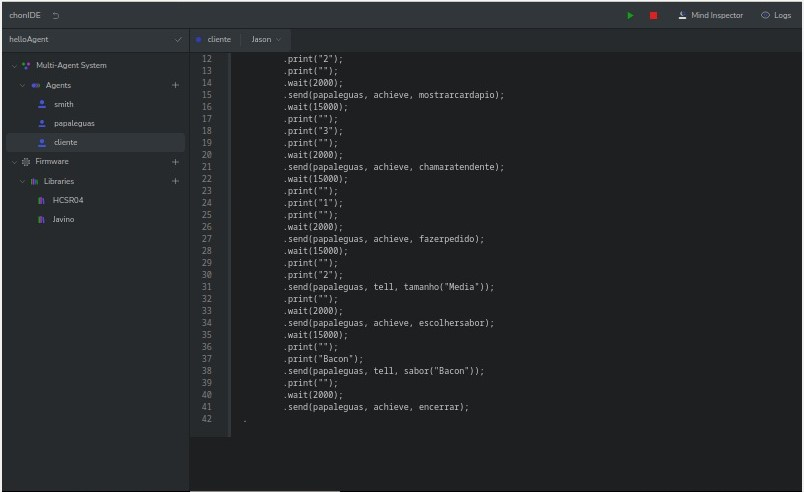
\includegraphics[width=1\textwidth]{figures/imagem08.jpeg}
        \caption{Codificação 4}
        \label{fig:imagem8}
    \end{figure}
    

    \newpage 
    \vspace{10mm} 
    \section{Utilização}

    \begin{figure}[!ht]
        \centering
        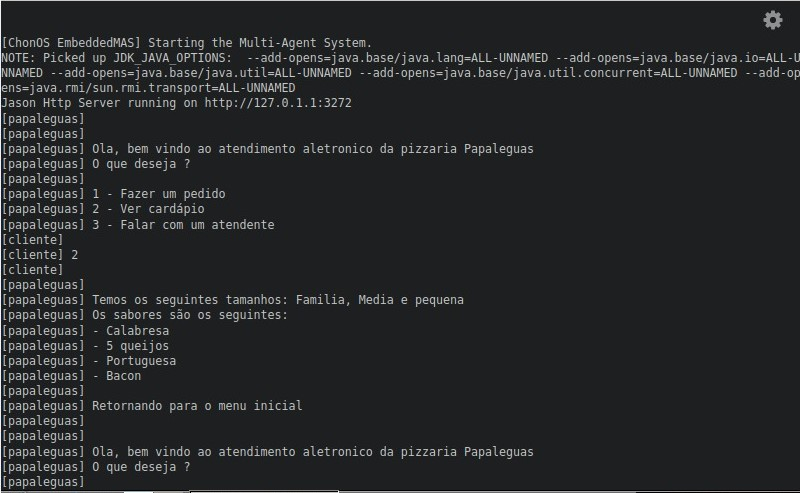
\includegraphics[width=1\textwidth]{figures/imagem01.jpeg}
        \caption{Utilização 1}
        \label{fig:imagem5}
    \end{figure}

    \newpage

    \begin{figure}[!ht]
        \centering
        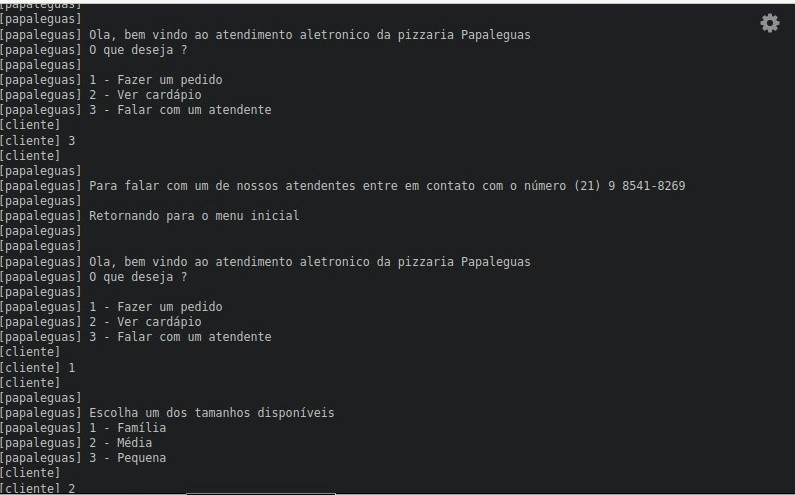
\includegraphics[width=1\textwidth]{figures/imagem02.jpeg}
        \caption{Utilização 2}
        \label{fig:imagem6}
    \end{figure}

    \begin{figure}[!ht]
        \centering
        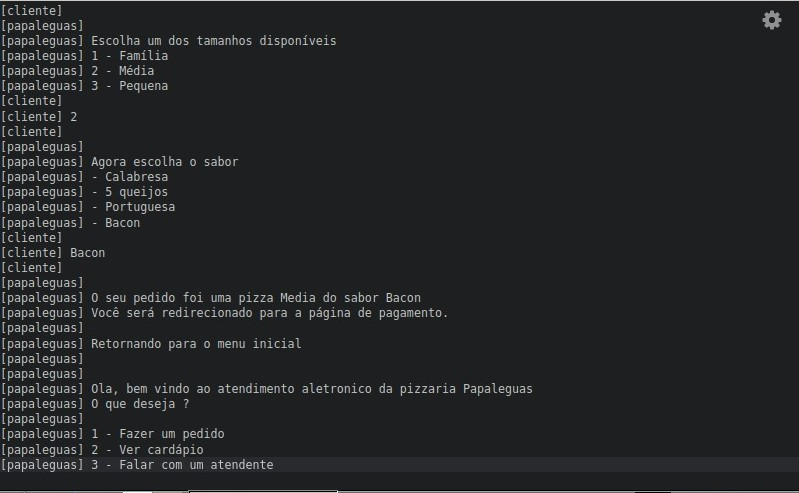
\includegraphics[width=1\textwidth]{figures/imagem03.jpeg}
        \caption{Utilização 3}
        \label{fig:imagem5}
    \end{figure}

    \newpage

    \begin{figure}[!ht]
        \centering
        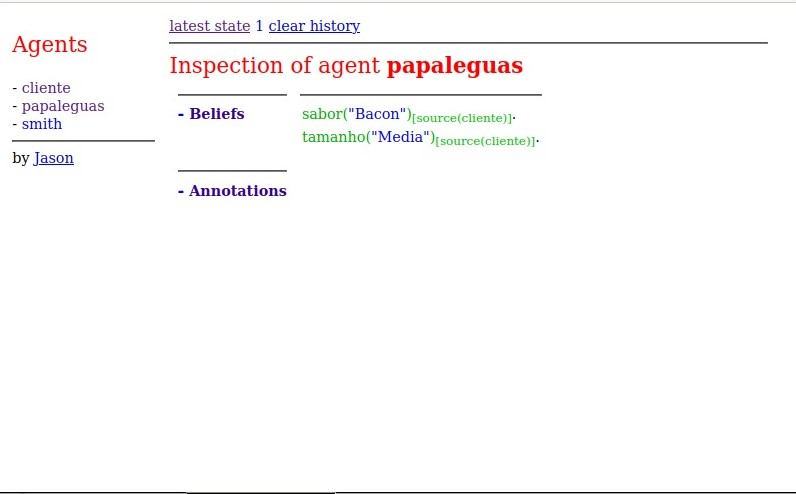
\includegraphics[width=1\textwidth]{figures/imagem04.jpeg}
        \caption{Utilização 4}
        \label{fig:imagem5}
    \end{figure}
    
\begin{thebibliography}{9}
\bibitem{wooldridge}
M. Wooldridge,
\textit{An Introduction to MultiAgent Systems},
John Wiley \& Sons, 2009.

\bibitem{bratman}
M. E. Bratman,
\textit{Intentions, Plans, and Practical Reason},
Harvard University Press, 1987.

\bibitem{jasondocumentation}
Equipe Jason,
\textit{Documentação do Jason},
Disponível em: \url{http://jason.sourceforge.net/}, 2023, Acesso em: 27 de setembro de 2023.

\end{thebibliography}

\end{document}
